\documentclass[a4paper,11pt]{article}
\usepackage[margin=25mm]{geometry}
\usepackage{fontspec}
\usepackage[english,russian]{babel}
\IfFontExistsTF{Liberation Serif}{\setmainfont{Liberation Serif}}{\setmainfont{Times New Roman}}
\IfFontExistsTF{Liberation Sans}{\setsansfont{Liberation Sans}}{\setsansfont{Arial}}
\IfFontExistsTF{DejaVu Sans Mono}{\setmonofont{DejaVu Sans Mono}[Scale=0.82]}{\setmonofont{Consolas}[Scale=0.82]}
\usepackage{amsmath,amssymb,amsthm,graphicx,booktabs,float}
\usepackage[hidelinks,unicode]{hyperref}
\setlength{\emergencystretch}{3em}
\newtheorem{theorem}{Теорема}[section]
\newtheorem{lemma}[theorem]{Лемма}
\newtheorem{proposition}[theorem]{Утверждение}
\newtheorem{corollary}[theorem]{Следствие}
\hypersetup{pdftitle={Метод Франк-Вульф при гладкости через зазор},pdfauthor={Ярослав П. Ляхов и Степан А. Суворов}}
\title{Метод Франк-Вульф при гладкости через зазор}
\author{Ярослав П. Ляхов \and Степан А. Суворов}
\date{14 ноября 2026 (редакция v20)}
\begin{document}
\maketitle
\begin{abstract}
Рассматривается условие кривизны
$\|\nabla^2f(x)\|\le L_0+L_1G(x)$ на допустимом множестве,
где $G$ обозначает полный зазор метода Франк-Вульф.
Доказаны оценка роста зазора вдоль выбранного направления,
экспоненциальная верхняя модель и логарифмический шаг с гарантией спуска.
Шаг не использует значение минимума или параметр квазар-выпуклости.
Для квазар-выпуклых функций накопленная вычисляемая нижняя граница
даёт конечную остановку и разделяет вклады
$L_0/\varepsilon$ и $L_1\log(1/\varepsilon)$.
Получена линейная сходимость при $L_0=0$, а также на сильно выпуклой
области при ненулевом градиенте в минимуме.
Для обычного FW с поиском Армихо доказан тот же порядок числа обновлений
при дополнительных пробных вычислениях функции. Получены явные параметры
из данных многомерной пуассоновской регрессии. Установлена связь с известными
условиями гладкости через норму градиента и условиями роста.
Экспоненциальный пример разделяет явный шаг и короткий шаг с фиксированной
общей константой $L$, хотя обычный полный шаг сразу решает этот пример.
Сравнение на синтетических задачах регрессии учитывает отдельные стоимости
оракулов и случаи, когда адаптивные конкуренты быстрее.
\end{abstract}
\section{Задача и доступные вычисления}
В минимуме на множестве норма градиента может не обращаться в ноль.
Полный зазор метода Франк-Вульф учитывает допустимые направления
и в минимуме равен нулю. Поэтому мы включаем зазор в условие
кривизны, выводим допустимый шаг спуска, а затем используем
квазар-выпуклость для оценки ошибки по функции.

Пусть $Q\subset\mathbb R^n$ является непустым компактным выпуклым
множеством, $\operatorname{diam}Q\le D$, $D>0$. Функция $f$
дважды непрерывно дифференцируема в окрестности $Q$.
Зафиксируем её минимизатор $x^*\in Q$. Нормы векторов евклидовы,
нормы матриц спектральны. Доступны значения функции, её градиенты
и точная минимизация линейной функции по всему $Q$.
В текущей точке $x$ вычисляем
\begin{equation}\label{eq:gap}
 s\in\arg\min_{v\in Q}\langle\nabla f(x),v\rangle,\qquad
 d=s-x,\qquad
 G(x)=\langle\nabla f(x),x-s\rangle
     =\max_{v\in Q}\langle\nabla f(x),x-v\rangle.
\end{equation}
Предположим, что
\begin{equation}\label{eq:gap_smoothness}
 \|\nabla^2f(x)\|\le L_0+L_1G(x)\quad(x\in Q),
 \qquad L_0,L_1\ge0.
\end{equation}
Это условие зависит от допустимого множества. В частности,
$L_1D^2$ является безразмерной величиной; множитель $D$ в оценке
роста зазора ниже необходим.

Для сходимости к глобальному минимуму используем
$\gamma$-квазар-выпуклость относительно $x^*$:
\begin{equation}\label{eq:quasar}
 \gamma\bigl(f(x)-f(x^*)\bigr)
       \le\langle\nabla f(x),x-x^*\rangle\quad(x\in Q),
 \qquad 0<\gamma\le1.
\end{equation}
Для выпуклой функции подходит $\gamma=1$. Это условие допускает
и невыпуклые функции; пример приведён в разделе~\ref{sec:examples}.
Для шага нужны верные $L_0,L_1,D$, а для проверки точности по
функции дополнительно используется $\gamma$. Точка $x^*$ и
значение $f(x^*)$ алгоритму не передаются.

Необходимое условие минимума на множестве даёт $G(x^*)=0$,
в том числе при $\nabla f(x^*)\ne0$.
Из \eqref{eq:gap} и \eqref{eq:quasar} следует
\begin{equation}\label{eq:certificate}
 0\le f(x)-f(x^*)\le \frac{G(x)}{\gamma}.
\end{equation}
Зазор ограничивает ошибку по функции сверху. Обратная оценка
из одной лишь квазар-выпуклости не следует.

\subsection{Связь с литературой и границы вклада}
Полный зазор и оценка ошибки через него стандартны~\cite{jaggi}.
Модель кривизны через норму градиента и анализ Выгузова и
Стонякина~\cite{vyguzov}, опубликованные также совместно с
Гасниковым~\cite{vyguzovjournal}, мотивируют рассмотрение
\eqref{eq:gap_smoothness}. Мартинес-Рубио~\cite{quasar} уже изучает
ограниченную квазар-выпуклую оптимизацию методом Франк-Вульф;
теорема~9 даёт $6LD^2/((k+1)\gamma^2)$ при обычной гладкости.
Таким образом, квазар-выпуклый вариант FW и множитель $\gamma^{-2}$
не являются новыми результатами настоящей работы.

Используемый ниже накопленный сертификат тоже имеет известный
выпуклый аналог: при $\gamma=1$ он точно совпадает с best primal-dual gap
из раздела~2.2 работы Wirth, Pe\~na и Pokutta~\cite{wirth}.
Условия роста в этой работе связывают остаток линейной модели со
степенями $G$. В разделе~\ref{sec:structure} установлена явная связь
с нашим предположением. Мы применяем сертификат к анализу выбранного
шага при $0<\gamma\le1$, не заявляя новый выпуклый сертификат.

Для сравнения шагов существенны адаптивные альтернативы.
Backtracking FW оценивает кривизну проверками значений функции~\cite{pedregosa},
а auto-conditioned FW использует кривизну в пробной точке без
внутреннего поиска~\cite{acfw}. Расширения на conditional gradient
без поиска шага рассматриваются и в~\cite{yagishita}.
Адаптивные шаги Брегмана используют другую модель --- относительную
гладкость~\cite{bregman}. Эти предположения не отождествляются с
\eqref{eq:gap_smoothness}.

\begin{table}[ht]
\centering\small
\caption{Место настоящего анализа. Константы разных моделей имеют
разный смысл; таблица не ранжирует методы.}
\begin{tabular}{p{.23\linewidth}p{.34\linewidth}p{.34\linewidth}}
\toprule
Анализ & Данные о кривизне или росте & Существенное отличие\\
\midrule
Norm-based FW~\cite{vyguzov} & $K_0+K_1\|\nabla f\|$ & Явный короткий шаг через норму градиента\\
Квазар-выпуклый FW~\cite{quasar} & Общая константа $L$ & Известная оценка при ограничениях\\
Open-loop FW~\cite{wirth} & Остаток модели через $G^r$ & Известный накопленный выпуклый сертификат\\
Адаптивный FW~\cite{pedregosa,acfw} & Информация в пробных точках & Не требует заданных $L_0,L_1$\\
Настоящий анализ & $L_0+L_1G$ & Перенос кривизны, минимум модели и сертифицированная остановка\\
\bottomrule
\end{tabular}
\end{table}

Вклад работы состоит в выводе и анализе этой модели: лемме переноса
вдоль направления, логарифмическом минимизаторе модели, раздельных
вкладах $L_0/\varepsilon$ и $L_1\log(1/\varepsilon)$ и проверяемых
примерах. Показано также, что обычное правило Армихо сохраняет тот же
порядок числа обновлений. Явный шаг экономит пробные вычисления
функции при известных допустимых параметрах; всеобщее численное
превосходство над адаптивным FW не утверждается.

\section{Две леммы и вычисляемый шаг}
Две леммы этого раздела используют \eqref{eq:gap_smoothness},
но не требуют выпуклости или квазар-выпуклости функции $f$.

\begin{lemma}[Рост зазора и верхняя модель]\label{lem:transport}
Пусть $s,d$ заданы в \eqref{eq:gap}. Для $0\le t\le1$ верно
\begin{align}
 G(x+td)&\le(1-t)G(x)
    +D\|d\|\int_0^t\bigl(L_0+L_1G(x+ud)\bigr)\,du,
       \label{eq:transport}\\
 L_0+L_1G(x+td)&\le
      \bigl(L_0+L_1G(x)\bigr)e^{L_1D\|d\|t}.
       \label{eq:transport_exp}
\end{align}
Поэтому для $0\le\alpha\le1$
\begin{equation}\label{eq:upper_model}
 f(x+\alpha d)\le f(x)-\alpha G(x)
 +(L_0+L_1G(x))\|d\|^2
       \int_0^\alpha(\alpha-t)e^{L_1D\|d\|t}\,dt.
\end{equation}
\end{lemma}
\begin{proof}
Для любого $v\in Q$ раскроем скалярное произведение относительно $x$:
\[
 \langle\nabla f(x+td),x+td-v\rangle
 \le G(x)-tG(x)
       +D\|\nabla f(x+td)-\nabla f(x)\|.
\]
Берём максимум по $v$ и интегрируем гессиан вдоль отрезка.
Получаем \eqref{eq:transport}. Отбрасываем неположительное
слагаемое $-tG(x)$ и применяем неравенство Гронуолла к
$L_0+L_1G(x+td)$; это даёт \eqref{eq:transport_exp}.
При $L_1=0$ оценка непосредственна.
Формула Тейлора с интегральным остатком даёт \eqref{eq:upper_model},
поскольку
$|d^\top\nabla^2f(x+td)d|\le\|\nabla^2f(x+td)\|\|d\|^2$.
\end{proof}

Экспонента в \eqref{eq:upper_model} ограничивает рост кривизны
при движении. Квадрат $\|d\|^2$ возникает из второй производной
вдоль направления. Оба множителя получены в доказательстве.
Выбранное направление существенно. Например, для
$f(t)=t+t^3/6$ на $[0,1]$ выполнено $|f''(t)|\le G(t)$,
однако $G(0)=0$ и $f(1)>f(0)+f'(0)$.
Поэтому верхнюю модель с начальным коэффициентом $L_0+L_1G(x)$
нельзя без изменения переносить на произвольную пару точек $x,y$.

\paragraph{Правило шага.}
При $G(x)>0$ и $L_1>0$ минимизируем правую часть
\eqref{eq:upper_model} на $[0,1]$:
\begin{equation}\label{eq:log_step}
 \boxed{\displaystyle
 \alpha=\min\left\{1,\,
 \frac{1}{L_1D\|d\|}
 \log\left(1+
 \frac{L_1D\,G(x)}
 {(L_0+L_1G(x))\|d\|}\right)\right\}.}
\end{equation}
Здесь и далее $\log$ означает натуральный логарифм.
При $L_1=0<L_0$ используем непрерывный предел
$\alpha=\min\{1,G(x)/(L_0\|d\|^2)\}$.
При $L_0=L_1=0$ берём $\alpha=1$: функция на $Q$ аффинна.
При $G(x)=0$ останавливаемся до вычисления дробей.

\begin{lemma}[Спуск]\label{lem:descent}
Указанный шаг удовлетворяет
\begin{equation}\label{eq:descent}
 f(x+\alpha d)\le f(x)-\frac{\alpha G(x)}2.
\end{equation}
Кроме отдельно разобранного аффинного случая,
\begin{equation}\label{eq:step_lower}
 \alpha\ge
 \min\left\{1,
   \frac{(\log2)G(x)}{(L_0+L_1G(x))D^2}\right\}.
\end{equation}
\end{lemma}
\begin{proof}
Только для этого скалярного вычисления положим
$b=L_1D\|d\|>0$. Интеграл в \eqref{eq:upper_model} равен
$(e^{b\alpha}-1-b\alpha)/b^2$.
Производная верхней модели имеет вид
\[
 -G(x)+(L_0+L_1G(x))\|d\|^2
             \frac{e^{b\alpha}-1}{b}.
\]
Её ноль даёт \eqref{eq:log_step}. В минимизаторе с ограничением
$\alpha\le1$ производная неположительна.
Функция $(e^{bt}-1)/b$ выпукла и равна нулю при $t=0$.
Поэтому её интеграл на $[0,\alpha]$ не больше половины произведения
$\alpha$ на значение в правом конце. Подставляем это в
\eqref{eq:upper_model} и получаем \eqref{eq:descent}.

Для \eqref{eq:step_lower} временно положим
$r=\|d\|/D\le1$ и $q=L_1G(x)/(L_0+L_1G(x))\le1$.
Неограниченный шаг равен $\log(1+q/r)/(L_1D^2r)$, причём
\[
 \log(1+q/r)\ge\log(1+q)\ge q\log2\ge qr\log2.
\]
Среднее неравенство следует из вогнутости логарифма.
При $L_1=0$ оба утверждения следуют из квадратичной модели.
\end{proof}

В шаге через норму градиента из~\cite{vyguzov} длина шага
ограничивает экспоненту числом $e$. Формула~\eqref{eq:log_step}
сразу минимизирует экспоненциальную модель. Логарифм обеспечивает
\[
 e^{L_1D\|d\|\alpha}-1
 \le\frac{L_1D\,G(x)}{(L_0+L_1G(x))\|d\|}.
\]
Именно это неравенство используется в доказательстве спуска.

\paragraph{Алгоритм и остановка.}
Зададим точность $\varepsilon>0$.
В каждой посещённой точке $x_k$ вычисляем $f(x_k)$, градиент
и линейный минимум по всему $Q$. Сохраняем
\begin{equation}\label{eq:stop}
 \ell_k=\max_{0\le j\le k}
        \left\{f(x_j)-\frac{G(x_j)}{\gamma}\right\},
 \qquad \text{остановка при } f(x_k)-\ell_k\le\varepsilon.
\end{equation}
Иначе полагаем $x_{k+1}=x_k+\alpha_kd_k$, используя
\eqref{eq:log_step} или указанные предельные случаи.
Каждое новое значение функции вычисляется один раз. Подбора шага нет.

\section{Остановка и сходимость}
\label{sec:rates}
Шаг использует наблюдаемый зазор и не требует $\gamma$.
Известное значение $\gamma$ нужно для нижней границы в
\eqref{eq:stop}. Из квазар-выпуклости следует
\begin{equation}\label{eq:retained_bound}
 0\le f(x_k)-f(x^*)\le f(x_k)-\ell_k\le G(x_k)/\gamma.
\end{equation}

\begin{theorem}[Конечная остановка с гарантией точности]
\label{thm:gap_stopping}
При условиях \eqref{eq:gap_smoothness} и \eqref{eq:quasar}
алгоритм останавливается с $f(x_N)-f(x^*)\le\varepsilon$.
Если $G(x_0)>\gamma\varepsilon$, положим
$J=\lceil\log_2(G(x_0)/(\gamma\varepsilon))\rceil$.
Число шагов удовлетворяет
\begin{equation}\label{eq:gap_iteration_bound}
 N\le\left\lceil
 \frac{\max\{4,4L_1D^2/\log 2\}}{\gamma}\,J
 +\frac{16L_0D^2}{(\log 2)\gamma^2\varepsilon}
 \right\rceil.
\end{equation}
Вычислений функции, градиента и запросов линейной минимизации
ровно по $N+1$, включая последний запрос.
Если $G(x_0)\le\gamma\varepsilon$, алгоритм останавливается сразу.
\end{theorem}
\begin{proof}
При $L_0=L_1=0$ функция аффинна и нужен не более чем один полный шаг.
В остальных случаях из \eqref{eq:step_lower} и \eqref{eq:descent} следует
\begin{equation}\label{eq:gap_progress}
 f(x_k)-f(x_{k+1})\ge
 \min\left\{\frac{G(x_k)}2,
 \frac{(\log 2)G(x_k)^2}{2D^2(L_0+L_1G(x_k))}\right\}.
\end{equation}
Значение функции убывает, а $\ell_k$ возрастает, поэтому
$f(x_k)-\ell_k$ убывает. Положим $b_j=G(x_0)/(\gamma2^j)$,
$0\le j<J$. Каждый шаг до остановки отнесём к фазе
$b_j/2<f(x_k)-\ell_k\le b_j$.
В этой фазе \eqref{eq:retained_bound} даёт $G(x_k)>\gamma b_j/2$.
Функция $t^2/(L_0+L_1t)$ возрастает при $t>0$, поэтому каждый
такой шаг уменьшает значение функции не меньше чем на
\[
 \min\left\{\frac{\gamma b_j}{4},
 \frac{(\log 2)\gamma^2b_j^2}{8D^2(L_0+L_1\gamma b_j/2)}\right\}.
\]
Суммарное уменьшение на шагах, начинающихся в фазе, не больше
истинной ошибки при входе, то есть не больше $b_j$.
Сюда входит и последний шаг, выводящий из фазы: его конечная
точка допустима. Поэтому число шагов в фазе не больше
\[
 \max\left\{\frac4\gamma,
 \frac{8L_0D^2}{(\log 2)\gamma^2b_j}
 +\frac{4L_1D^2}{(\log 2)\gamma}\right\}.
\]
Суммирование и $\sum_{j<J}b_j^{-1}<2/\varepsilon$ доказывают
\eqref{eq:gap_iteration_bound}. Та же конечная граница верна для
каждого незавершённого начала процесса, поэтому бесконечный процесс
без остановки невозможен. В каждой посещённой точке по одному разу
вычисляются функция, градиент и линейный минимум.
Явный шаг \eqref{eq:log_step} не требует пробных вычислений функции.
\end{proof}

\subsection{Случай \texorpdfstring{$L_0=0$}{L0=0}}
\begin{corollary}[Геометрическая сходимость]\label{cor:pure_gap_linear}
Если $L_0=0<L_1$, положим
\[
 \underline\alpha_0=\min\{1,(\log 2)/(L_1D^2)\}.
\]
Для каждой вычисленной точки выполнено
\begin{align*}
 f(x_k)-f(x^*)&\le
 (1-\gamma\underline\alpha_0/2)^k\bigl(f(x_0)-f(x^*)\bigr),\\
 f(x_k)-\ell_k&\le
 (1-\gamma\underline\alpha_0/2)^k G(x_0)/\gamma.
\end{align*}
Если начальная проверка не дала остановки, достаточно не более
\[
 \left\lceil\frac{\log(G(x_0)/(\gamma\varepsilon))}
 {-\log(1-\gamma\underline\alpha_0/2)}\right\rceil
\]
шагов.
\end{corollary}
\begin{proof}
Граница шага даёт $\alpha_k\ge\underline\alpha_0$, поэтому
уменьшение функции не меньше $\underline\alpha_0G(x_k)/2$.
Для первой рекуррентной оценки используем \eqref{eq:quasar},
а для второй \eqref{eq:retained_bound} и $\ell_{k+1}\ge\ell_k$.
\end{proof}
Здесь $\nabla^2f(x^*)=0$ следует из $G(x^*)=0$.
Невыпуклый пример в разделе~\ref{sec:examples} обладает этим свойством
и ненулевым градиентом в минимуме.

\subsection{Сильно выпуклая допустимая область}
Используем определение из \cite{vyguzov}: множество $Q$ сильно
выпукло с константой $\lambda>0$, если для любых $u,v\in Q$
замкнутый шар радиуса $\lambda\|u-v\|^2$ с центром $(u+v)/2$
содержится в $Q$. Это условие на область, а не сильная выпуклость
целевой функции.

\begin{theorem}[Ненулевой градиент в минимуме и линейная скорость]
\label{thm:strong_set_linear}
Пусть дополнительно $Q$ сильно выпукло и $\nabla f(x^*)\ne0$.
Тогда минимум $x^*$ единственен и
\[
 c:=\min_{x\in Q}\|\nabla f(x)\|>0.
\]
Положим
\[
 \underline\alpha_{\rm sc}=
 \min\left\{1,\left(\frac{L_0}{2\lambda c}+2L_1D^2\right)^{-1}\right\},
\]
причём при нулевом знаменателе значение равно $1$. Тогда
\begin{align*}
 f(x_k)-f(x^*)&\le
 (1-\gamma\underline\alpha_{\rm sc}/2)^k
       \bigl(f(x_0)-f(x^*)\bigr),\\
 f(x_k)-\ell_k&\le
 (1-\gamma\underline\alpha_{\rm sc}/2)^k G(x_0)/\gamma.
\end{align*}
Алгоритм не использует ни $c$, ни $\lambda$; они нужны только
для этой оценки скорости.
\end{theorem}
\begin{proof}
Если бы $y$ было другим минимумом, условие \eqref{eq:quasar}
означало бы, что отношение
\[
 \frac{f(x^*+t(y-x^*))-f(x^*)}{t^\gamma}
\]
не убывает при $0<t\le1$. Оно неотрицательно и равно нулю при
$t=1$, поэтому функция постоянна на всём отрезке и
$\langle\nabla f(x^*),y-x^*\rangle=0$.
Однако условие на шар и необходимое условие минимума на $Q$ дают
\[
 \langle\nabla f(x^*),y-x^*\rangle
 \ge2\lambda\|\nabla f(x^*)\|\|y-x^*\|^2>0
\]
при $y\ne x^*$. Значит, минимум единственен.
Нулевой градиент в любой точке $Q$ по \eqref{eq:quasar} означал бы
ещё один минимум. Теперь непрерывность и компактность дают $c>0$.

Та же конструкция с шаром в точке линейного минимума даёт
\[
 G(x_k)\ge2\lambda\|\nabla f(x_k)\|\|d_k\|^2
           \ge2\lambda c\|d_k\|^2.
\]
При $L_0=L_1=0$ имеем $\alpha_k=1$. В остальных случаях используем
$\log(1+t)\ge t/(1+t)$ в \eqref{eq:log_step}
или указанный предел при $L_1=0$:
\[
 \alpha_k\ge\min\left\{1,
 \frac{G(x_k)}{(L_0+L_1G(x_k))\|d_k\|^2
                      +L_1D\|d_k\|G(x_k)}\right\}
 \ge\underline\alpha_{\rm sc}.
\]
Здесь $\|d_k\|\le D$, а предыдущее неравенство ограничивает
знаменатель, делённый на $G(x_k)$, числом
$L_0/(2\lambda c)+2L_1D^2$.
Обе рекуррентные оценки следуют так же, как в
следствии~\ref{cor:pure_gap_linear}.
\end{proof}

\subsection{Гарантии обычного правила Армихо}\label{sec:armijo}
Рассмотрим известное правило достаточного убывания: в каждой точке
начинаем с $\alpha=1$ и умножаем шаг на фиксированное
$\beta\in(0,1)$ до выполнения
\begin{equation}\label{eq:armijo}
 f(x+\alpha d)\le f(x)-\alpha G(x)/2.
\end{equation}
Используем тот же сертификат \eqref{eq:stop} и сохраняем принятое
значение функции. Это обычный поиск Армихо, не новый алгоритм FW;
для него не нужны $L_0,L_1,D$.

\begin{proposition}[Сертифицированная сложность метода сравнения]
\label{prop:armijo}
В условиях теоремы~\ref{thm:gap_stopping} обозначим через
$\alpha_{\log}(x)$ шаг \eqref{eq:log_step} вместе с предельными случаями.
Поиск конечен, а принятый шаг удовлетворяет
$\alpha\ge\beta\alpha_{\log}(x)$.
При $G(x_0)>\gamma\varepsilon$ число обновлений ограничено:
\[
 N\le\left\lceil\frac1\beta\left[
 \frac{\max\{4,4L_1D^2/\log2\}}\gamma J
 +\frac{16L_0D^2}{(\log2)\gamma^2\varepsilon}
 \right]\right\rceil,
 \qquad J=\left\lceil\log_2\frac{G(x_0)}{\gamma\varepsilon}\right\rceil.
\]
Вне аффинного случая положим
\[
 a_\varepsilon=\min\left\{1,
 \frac{(\log2)\gamma\varepsilon}
 {D^2(L_0+L_1\gamma\varepsilon)}\right\},\qquad
 T_\varepsilon=1+\left\lceil\frac{\log(1/a_\varepsilon)}{\log(1/\beta)}\right\rceil.
\]
Число вычислений градиента и линейного минимума равно $N+1$,
а число вычислений функции не превосходит $1+NT_\varepsilon$.
В аффинном случае для единственного возможного обновления
достаточно одной пробы.
\end{proposition}
\begin{proof}
Доказательство леммы~\ref{lem:descent} применимо к каждому
$0<\alpha\le\alpha_{\log}(x)$: производная модели остаётся
неположительной, а та же оценка интеграла даёт \eqref{eq:armijo}.
Поэтому первая точка геометрической сетки, не превосходящая
$\alpha_{\log}(x)$, будет принята, если раньше не принят больший шаг.
Это доказывает конечность поиска и нижнюю границу шага.
Фазовое доказательство теоремы~\ref{thm:gap_stopping} применяется
с уменьшением гарантированного спуска в $\beta$ раз.
До остановки $G(x)>\gamma\varepsilon$. Монотонность
$G/(L_0+L_1G)$ и \eqref{eq:step_lower} дают
$\alpha_{\log}(x)\ge a_\varepsilon$, откуда достаточно
$T_\varepsilon$ проб. Принятое значение функции используется
повторно при переходе к новой точке.
\end{proof}
При $L_0=0$ сертификат за обновление сокращается не хуже, чем
в $1-\beta\gamma\underline\alpha_0/2$ раза. В условиях
теоремы~\ref{thm:strong_set_linear} аналогичный множитель равен
$1-\beta\gamma\underline\alpha_{\rm sc}/2$.
Следовательно, благоприятная оценка числа обновлений определяется
условием кривизны и не является исключительным свойством
логарифмической формулы. Её особенность --- гарантированный шаг
без отклонённых пробных вычислений функции.

\section{Область применимости условия кривизны}\label{sec:structure}
\subsection{Обычная гладкость и модель через норму градиента}
Поскольку $f$ дважды непрерывно дифференцируема в окрестности
компактного $Q$, общая граница $L=\max_{x\in Q}\|\nabla^2f(x)\|$
конечна. Польза нового условия состоит в параметрах и локальной
модели, а не в охвате функций без конечной константы гладкости на
данном фиксированном $Q$. Кроме того,
\[
 G(x)\le D\|\nabla f(x)\|,
 \qquad \|\nabla^2f(x)\|\le L_0+(L_1D)\|\nabla f(x)\|.
\]
Значит, гладкость через зазор влечёт оценку через норму градиента на $Q$.
Обратный переход с нулевым постоянным слагаемым неверен:
для $f(t)=e^t$ на $[0,R]$ выполнено $|f''|=|f'|$, но $G(0)=0$
и $f''(0)=1$. Поэтому любая допустимая пара параметров через зазор
в этом примере имеет $L_0\ge1$. В общем случае
$L_0\ge\|\nabla^2f(x^*)\|$.

\begin{proposition}[Ограничение режима с нулевым постоянным слагаемым]
\label{prop:rigidity}
Пусть \eqref{eq:gap_smoothness} выполнено при $L_0=0$.
Если $\nabla f(z)=0$ хотя бы в одной точке $z\in Q$, то
$\nabla f=0$ на $Q$ и $f$ постоянна на $Q$.
Выпуклость или квазар-выпуклость $f$ не требуется.
\end{proposition}
\begin{proof}
Зафиксируем $y\in Q$ и положим $u(t)=\|\nabla f(z+t(y-z))\|$.
Основная теорема анализа и $G\le D\|\nabla f\|$ дают
\[
 u(t)\le L_1D\|y-z\|\int_0^t u(s)\,ds.
\]
По неравенству Гронуолла $u=0$. Точка $y$ произвольна.
\end{proof}
Следовательно, непостоянная функция в этом режиме не может иметь
минимизатор с нулевым градиентом. В частности, исключён внутренний
минимум на полноразмерном множестве. Это ограничивает область
применимости следствия~\ref{cor:pure_gap_linear}.

\subsection{Связь с известными условиями роста}
Для выпуклой $f$ обозначим
$D_f(y,x)=f(y)-f(x)-\langle\nabla f(x),y-x\rangle$.
При $L_0=0<L_1$ лемма~\ref{lem:transport} даёт для $0\le\alpha\le1$
\[
 D_f(x+\alpha d,x)\le\frac{M\alpha^2}{2}G(x),
 \qquad M=L_1D^2e^{L_1D^2}.
\]
Достаточно ограничить экспоненту в \eqref{eq:upper_model} числом
$e^{L_1D^2}$ и проинтегрировать $\alpha-t$.
Это strong $(M,1)$-growth из~\cite{wirth}.
Такое сведение консервативно: возникает экспоненциальная зависимость
от $L_1D^2$, тогда как следствие~\ref{cor:pure_gap_linear} использует
нижнюю границу шага порядка $\min\{1,(L_1D^2)^{-1}\}$.
Сравниваются именно выписанные способы преобразования констант;
это не нижняя граница возможностей всех других методов или доказательств.

\subsection{Многомерный класс с явными параметрами}
Пусть $a_i\in\mathbb R^n$, $y_i\ge0$, $B=\max_i\|a_i\|>0$.
Рассмотрим отрицательное логарифмическое правдоподобие пуассоновской
модели без слагаемых, зависящих только от данных:
\begin{equation}\label{eq:poisson}
 f(x)=\frac1m\sum_{i=1}^m\bigl(e^{a_i^Tx}-y_i a_i^Tx\bigr),
 \qquad 0\in Q.
\end{equation}
При целых $y_i$ это задача регрессии счётных данных; оценка ниже
верна и для неотрицательных вещественных откликов.

\begin{proposition}[Параметры из наблюдаемых данных]\label{prop:poisson}
На любом компактном выпуклом $Q$, содержащем ноль, функция
\eqref{eq:poisson} удовлетворяет \eqref{eq:gap_smoothness} при
\begin{equation}\label{eq:poisson_constants}
 L_0=B^2\left(1+\frac{1}{2m}\sum_i y_i^2\right),
 \qquad L_1=B^2,\qquad \gamma=1.
\end{equation}
Минимизатор и значение минимума для этих констант не нужны.
Если $Q=\{x:\|x\|\le R\}$, то допустимы параметры модели через
норму градиента $K_0=L_0$, $K_1=RL_1$ и общая граница гессиана
\begin{equation}\label{eq:poisson_uniform}
 L=e^{BR}\|A\|_2^2/m,
\end{equation}
где строки $A$ равны $a_i^T$. Утверждается допустимость этих
границ, а не их минимальность.
\end{proposition}
\begin{proof}
При $y\ge0$ и любом $t\in\mathbb R$ верно
\begin{equation}\label{eq:poisson_scalar}
 e^t\le1+y^2/2+t(e^t-y).
\end{equation}
Если $t\le0$, то $(1-t)e^t+yt\le1$.
Если $t\ge0$, производная $(1-t)e^t$ равна $-te^t\le-t$,
поэтому $(1-t)e^t+yt\le1-t^2/2+yt\le1+y^2/2$.
При этом $\|\nabla^2f(x)\|\le B^2m^{-1}\sum_i e^{a_i^Tx}$.
Суммирование \eqref{eq:poisson_scalar} даёт
\[
 \|\nabla^2f(x)\|\le L_0+L_1\langle\nabla f(x),x\rangle
 \le L_0+L_1G(x),
\]
поскольку $0\in Q$.
На шаре $\langle\nabla f(x),x\rangle\le R\|\nabla f(x)\|$.
Наконец, из $a_i^Tx\le BR$ следует
$\nabla^2f(x)\preceq e^{BR}A^TA/m$.
\end{proof}
При ненулевом градиенте линейный оракул шара имеет вид
$s=-R\nabla f(x)/\|\nabla f(x)\|$ и в общем случае отличается от
минимизатора \eqref{eq:poisson}. Эти задачи не обладают вырожденным
свойством скалярных примеров ниже, где оракул сразу находит минимум.
Условия и параметры доказаны на всём $Q$; численные опыты лишь
проверяют их следствия в выбранных точках.

\section{Примеры и количественное сравнение}\label{sec:examples}
\subsection{Параметры через зазор и большая общая константа}
Рассмотрим
\begin{equation}\label{eq:exp_family}
 f_A(x,y)=e^x+Ay,\qquad
 Q=[0,R]\times[0,1],\qquad R,A>0,\qquad D=\sqrt{R^2+1}.
\end{equation}
Функция выпукла, минимум достигается в $(0,0)$, причём
$\nabla f_A(0,0)=(1,A)$.
Линейный минимум всегда равен $(0,0)$, поэтому
\[
 G(x,y)=xe^x+Ay,\qquad
 \|\nabla^2 f_A(x,y)\|=e^x\le1+xe^x\le1+G(x,y).
\]
Действительно, $(1-x)e^x$ не возрастает при $x\ge0$ и равна единице
в нуле. Значит, для всех $R,A$ подходят $L_0=L_1=1$,
а наименьшая общая граница гессиана на $Q$ равна $L=e^R$.

\begin{theorem}[Два правила шага на одном семействе]\label{thm:separation}
Начнём оба метода из $(R,0)$ в задаче \eqref{eq:exp_family}.
Если продолжать итерации без более ранней остановки с положительным
допуском, логарифмическое правило \eqref{eq:log_step} достигает точного
минимума не более чем за
\begin{equation}\label{eq:exp_upper}
 N_{\log}\le\left\lceil\frac{R\sqrt{R^2+1}}{\log2}\right\rceil
\end{equation}
шагов. Для обычного короткого шага
$\alpha=\min\{1,G/(L\|d\|^2)\}$ с $L=e^R$
достижение ошибки по функции не выше $\varepsilon>0$ требует
\begin{equation}\label{eq:exp_lower}
 N_L\ge\frac{e^R/(1+\varepsilon)-1}{e-1}.
\end{equation}
Точки, шаги, значения функции, зазоры, оценки ошибки и число
вычислений не зависят от $A$.
\end{theorem}
\begin{proof}
Все точки имеют $y=0$. Для логарифмического правила первая
координата обновляется по формуле
\[
 x_{\mathrm{next}}=\max\{0,x-h(x)\},\qquad
 h(x)=\frac1D\log\left(1+\frac{D}{x+e^{-x}}\right).
\]
На $[0,R]$ верно $x+e^{-x}\le R+e^{-R}\le D$.
Последнее следует из $e^R-e^{-R}\ge2R$: производная левой части
не меньше двух.
Поэтому $h(x)\ge(\log2)/D$, что доказывает \eqref{eq:exp_upper}.

Для обычного короткого шага
$x_{\mathrm{next}}=x-h$, где $h=\min\{x,e^{x-R}\}\le1$.
Из выпуклости экспоненты на $[0,1]$ следует
\[
 e^{-(x-h)}-e^{-x}
 =e^{-x}(e^h-1)
 \le(e-1)e^{-x}h\le(e-1)e^{-R}.
\]
В начале $e^{-x}=e^{-R}$. Ошибка не выше $\varepsilon$ требует
$e^{-x}\ge1/(1+\varepsilon)$, откуда получаем \eqref{eq:exp_lower}.
На грани $y=0$ значения функции, зазоры, направления и формулы
шага не зависят от $A$. То же верно для проверки \eqref{eq:stop}.
\end{proof}

При фиксированной точности верхняя граница для нового шага
имеет порядок $R^2$. Нижняя граница для обычного шага с $L=e^R$
имеет порядок $e^R$. Значения $L_0,L_1$ влияют на доказанную
оценку работы метода. Сравнивать лишь числа с разными
размерностями недостаточно.

\paragraph{Границы сравнения.}
В задаче \eqref{eq:exp_family} линейный оракул в любой точке возвращает
глобальный минимизатор. Поэтому обычный шаг $\alpha_k=2/(k+2)$,
считая $k$ от нуля, достигает минимума за одно обновление; то же
верно для точного поиска по отрезку. Теорема~\ref{thm:separation}
разделяет два конкретных правила шага и не является нижней границей
сложности всех вариантов FW или доказательством превосходства над
адаптивными конкурентами. Изменение $A$ при старте $(R,0)$ не создаёт
новых траекторий: это одномерная проверка чувствительности к нормальной
компоненте градиента.

\subsection{Невыпуклая функция с ненулевым градиентом в минимуме}
На $Q=[0,1]$ рассмотрим
\begin{equation}\label{eq:nonconvex}
 f(x)=\int_0^x e^{-2t^2}\,dt.
\end{equation}
Минимизатор $x^*=0$, производная $f'(0)=1$, а $f''(x)<0$ при $x>0$.
Кроме того,
\[
 G(x)=xe^{-2x^2},\qquad
 |f''(x)|=4G(x),\qquad
 xf'(x)\ge e^{-2}x\ge e^{-2}f(x).
\]
Условие \eqref{eq:gap_smoothness} выполнено при $L_0=0,L_1=4$,
а \eqref{eq:quasar} выполнено при $\gamma=e^{-2}$.
Это невыпуклый пример заявленного класса.

Из $x_0=1$ первый логарифмический шаг даёт
$x_1=1-(\log2)/4\in(1/2,1)$.
Функция $xe^{-2x^2}$ убывает по $x$ на $(1/2,1]$,
поэтому $G(x_1)>G(x_0)$, хотя $f(x_1)<f(x_0)$.
Именно поэтому доказательство остановки использует монотонную
величину $f(x_k)-\ell_k$ и не предполагает монотонности $G(x_k)$.
Норма градиента при приближении к минимуму на множестве растёт
к единице.

Здесь линейный оракул тоже возвращает минимизатор $0$, а точный
поиск по отрезку выбирает полный шаг. Пример проверяет принадлежность
невыпуклой функции классу при $L_0=0$ и немонотонность $G$,
но не демонстрирует сложную численную задачу.

\section{Воспроизводимые численные сравнения}\label{sec:experiments}
\subsection{Сохранённые аналитические проверки}
Фиксированные проверки используют \eqref{eq:exp_family} при
$R\in\{1,2,4,6,8\}$, $A\in\{1,1000\}$, старте $(R,0)$ и
$\varepsilon=10^{-6}$. Оба коротких шага используют \eqref{eq:stop}
с $\gamma=1$. Для Gap-log $L_0=L_1=1$, а для Global-$L$ ---
наименьшая общая константа $L=e^R$. Два значения $A$ дают одинаковые
траектории, а не независимые задачи. В таблицу~\ref{tab:endpoint}
включены методы с полным первым шагом, необходимые для интерпретации.
\begin{table}[ht]
\centering
\caption{Обновления на экспоненциальном примере. Последний столбец
следует из того, что линейный оракул возвращает минимизатор.
Запрос в конечной точке подтверждает остановку.}\label{tab:endpoint}
\begin{tabular}{rrrr}
\toprule
$R$ & Gap-log & Global-$L$ & Open-loop / точный поиск\\
\midrule
1 & 2 & 1 & 1\\
2 & 5 & 6 & 1\\
4 & 17 & 52 & 1\\
6 & 35 & 400 & 1\\
8 & 60 & 2976 & 1\\
\bottomrule
\end{tabular}
\end{table}
Ещё четыре проверки используют \eqref{eq:nonconvex}, функцию
$f(x)=x+x^2/2$ на $[0,1]$ из $1$, функцию $f(x)=x$ на том же
отрезке из $1$ и \eqref{eq:exp_family} при $R=4,A=1000$ из $(0,0)$.
Они дают $5,1,1,0$ обновлений. Все 24 исходных запуска проходят
проверки. Итоговые значения воспроизведены; отдельные элементы
траекторий отличаются последними цифрами округления между средами.
Побайтовое совпадение численных траекторий на разных платформах
не утверждается.

\subsection{Протокол многомерной регрессии}
Рассматривается \eqref{eq:poisson} на евклидовых шарах. Для
$n\in\{4,12\}$ и начальных состояний генератора $11,29,47$
строятся $m=12n$ независимых стандартных гауссовских строк,
нормированных до единичной евклидовой нормы. Следующий гауссовский
вектор масштабируется до нормы $1.2$ и обозначается $b$.
Генерируются целые отклики $y_i\sim\operatorname{Poisson}(e^{a_i^Tb})$.
Используются радиусы $R\in\{0.5,2,4\}$ и старты $0,Re_1,-Re_1$.
Шесть наборов данных, три радиуса и три старта дают 18 ограниченных
задач и 54 стартовые конфигурации. Радиусы и старты с общими данными
зависимы и не считаются независимыми статистическими наблюдениями.

У всех методов одинаковый сертификат \eqref{eq:stop}, $\gamma=1$,
$\varepsilon=10^{-4}$ и бюджет 20\,000 внешних попыток.
Параметры зафиксированы в \texttt{Code/benchmark\_multidim.py}
и записываются в протокол до вычислений. Матрицы и отклики сохранены.
Параметры через зазор и норму градиента берутся из
утверждения~\ref{prop:poisson}, общая граница --- из
\eqref{eq:poisson_uniform}. По результатам параметры не подбираются.

Сравниваются восемь правил. Gap-log использует \eqref{eq:log_step},
Global-$L$ --- $\min\{1,G/(L\|d\|^2)\}$, Open-loop --- $2/(k+2)$.
Armijo начинает с $1$ и делит шаг пополам до \eqref{eq:armijo}.
Backtracking проверяет квадратичную модель из~\cite{pedregosa}:
начальная оценка $M=1$, первая проба каждой итерации использует
$M/2$, при неудаче $M$ удваивается. Norm-based использует
$\min\{1,G/[e(K_0+K_1\|\nabla f\|)\|d\|^2]\}$ из~\cite{vyguzov}.
Line bisection проверяет производную в конце отрезка и при смене
знака делит интервал пополам до ширины $10^{-12}$; это численное
приближение точного поиска. AC-FW реализует алгоритмы~1--2 и
последовательность (6) при $\delta=1$ из~\cite{acfw}.
Его обязательный начальный переход к результату LMO учитывается
и может увеличить функцию. Используются собственные реализации,
а не программное обеспечение авторов цитируемых работ.

Счётчики функции, полного градиента и LMO увеличиваются при каждом
фактическом вызове. Учтены отклонённые пробы и градиенты внутри
бисекции. Принятые значения функции используются повторно;
после отклонения AC-пробы сохраняются неизменные градиент и атом.
Минимум решателям не передаётся. Отдельно метод SLSQP строит
диагностический интервал $[f(z)-G(z),f(z)]$; его наибольшая вычисленная
ширина равна $2.75\cdot10^{-7}$. По записанному допуску семь из
18 эталонных решений граничные, одиннадцать внутренние. Это
диагностика с плавающей точкой, а не точное доказательство оптимальности.

\subsection{Результаты и вычислительные затраты}
Записано 432 запуска. Gap-log и ещё шесть методов достигают точности
во всех 54 конфигурациях; Open-loop исчерпывает бюджет в девяти
конфигурациях при $n=4,R=4$. Их конечные сертификаты находятся
между $1.07\cdot10^{-4}$ и $1.80\cdot10^{-4}$, и эти запуски
сохранены во всех сводках. В таблице~\ref{tab:costs} приведены медианы
по всем 54 конфигурациям, включая концы незавершённых запусков.
Для такого метода эти затраты нельзя интерпретировать как
гарантированную стоимость достижения точности.

\begin{table}[ht]
\centering\small
\caption{Зарегистрированные затраты: успешные запуски, обновления $N$,
вызовы функции $F$, градиента $H$, LMO $V$ и миллисекунды.
Время --- сначала медиана трёх последовательных повторов без записи
траектории для каждой конфигурации, затем медиана по конфигурациям;
проверки и запись файлов исключены.}\label{tab:costs}
\begin{tabular}{lrrrrrr}
\toprule
Правило & Успех & $N$ & $F$ & $H$ & $V$ & мс\\
\midrule
\csname @@input\endcsname multidim_table.tex
\bottomrule
\end{tabular}
\end{table}

\begin{table}[ht]
\centering\small
\caption{Медианы зарегистрированных обновлений при каждом радиусе
по 18 стартовым конфигурациям. Все незавершённые запуски
Open-loop относятся к $R=4$.}\label{tab:radius}
\begin{tabular}{lrrr}
\toprule
Правило & $R=0.5$ & $R=2$ & $R=4$\\
\midrule
\csname @@input\endcsname radius_table.tex
\bottomrule
\end{tabular}
\end{table}

При $R=4$ Gap-log улучшает медиану обновлений относительно
используемой общей границы: 216.5 против 819. При двух меньших
радиусах Global-$L$ дешевле. Backtracking и AC-FW на этой выборке
существенно дешевле Gap-log. Armijo использует меньше градиентов
и LMO, но оплачивает повторные вычисления функции; бисекция
требует много градиентов. Разделение оракульных затрат меняет
интерпретацию числа обновлений. Опыты показывают ограничения
фиксированной общей границы в некоторых режимах, но не превосходство
над адаптивными альтернативами.

\begin{figure}[ht]
\centering
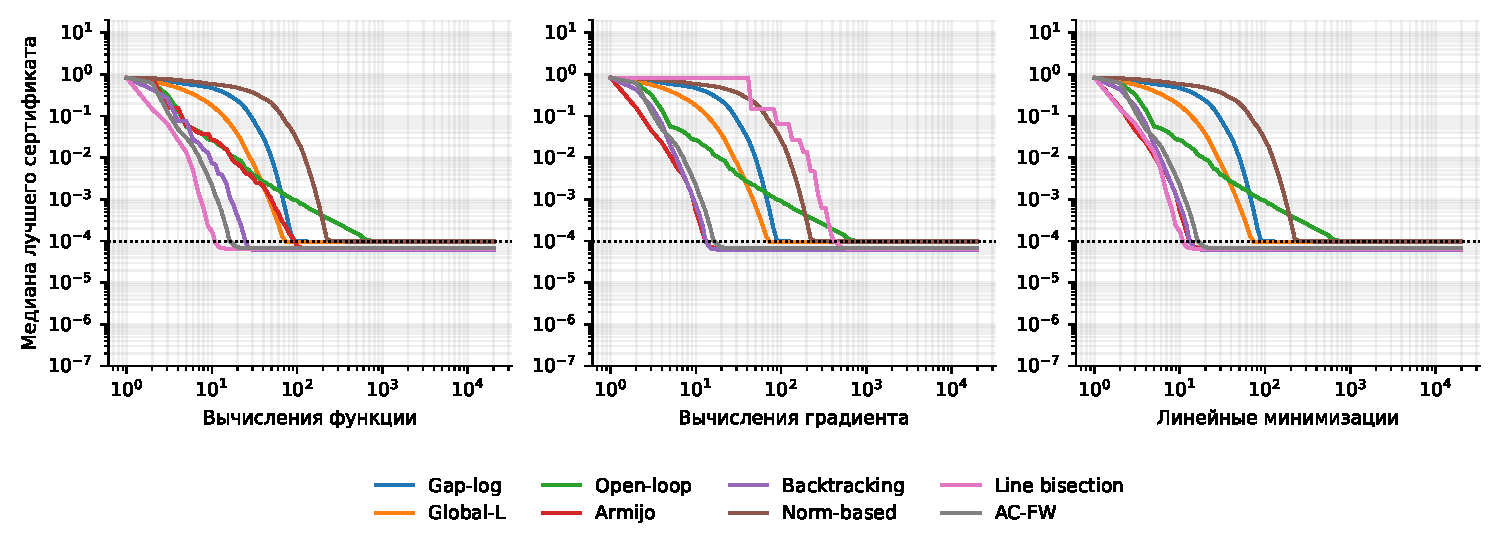
\includegraphics[width=\linewidth]{../figures/multidim_ru.pdf}
\caption{Медиана лучшего записанного сертификата при отдельных
оракульных бюджетах на тех же 54 конфигурациях. После остановки
или исчерпания бюджета сохраняется последнее лучшее значение.
Пунктир соответствует $10^{-4}$. Панели используют разные единицы
стоимости; они не суммируются.}\label{fig:cost_curves}
\end{figure}

\paragraph{Воспроизведение и проверки.}
\texttt{Code/benchmark\_gap.py} воспроизводит исходные проверки,
а \texttt{Code/benchmark\_multidim.py} сохраняет многомерные точки,
параметры, статусы и счётчики оракулов.
\texttt{Code/report\_results.py} строит таблицы и рисунки из готовых
данных без решения новых задач. Аудит 340\,433 записанных точек
проверяет допустимость, согласованность нижних границ с диагностическими
интервалами, применимые оценки спуска и шага, учёт оракулов.
Границы гессиана дополнительно проверяются не более чем в 25 точках
каждого запуска; их глобальное обоснование --- утверждение~\ref{prop:poisson},
а не эта выборочная проверка.
Восемь отдельных тестов проверяют производные конечными разностями,
скалярное неравенство, масштабирование, фактические вызовы интерфейсов,
остановку в начальном минимуме, пробы Армихо, бисекцию и неоптимальность
результата оракула. Проходят и 13 исходных символьных тождеств.
Зависимости и команды приведены в сопровождающем архиве.

\section{Ограничения и интерпретация}
Гарантии предполагают точные градиенты и полную линейную минимизацию.
Неточные и стохастические оракулы требуют дополнительных слагаемых
ошибки и здесь не рассматриваются. Для логарифмического шага нужны
допустимые $L_0,L_1,D$, а для сертифицированной точности по функции
ещё и допустимый $\gamma$. Утверждение~\ref{prop:poisson} даёт эти
величины для конкретного класса, но не решает задачу их проверки
для произвольных моделей.

На компактном множестве наши предположения уже влекут обычную
гладкость. Существенна полезность параметров через зазор, а не
существование глобальной константы $L$. Утверждение~\ref{prop:rigidity}
ограничивает режим $L_0=0$: он не описывает непостоянную функцию с
нулевым градиентом в минимуме. Условие ненулевого градиента в
теореме~\ref{thm:strong_set_linear} содержательно.

Опыты выполнены на небольших синтетических задачах регрессии.
Общие и norm-based константы являются допустимыми аналитическими
границами, а не оптимизированными значениями. Время зависит от
оборудования и реализации. Результаты не доказывают всеобщего
превосходства, оптимальности зависимости от $\gamma$ или совпадения
верхних и нижних оценок сложности. Утверждение~\ref{prop:armijo}
прямо показывает, что известное адаптивное правило сохраняет тот же
порядок числа принятых обновлений. Вклад состоит в анализе кривизны
через зазор с явными параметрами и шаге, минимизирующем верхнюю модель
без отклонённых вычислений функции.

\paragraph{Вычислительные инструменты.}
ИИ использован при выводах, проверках, подготовке кода и текста.
За математические утверждения и результаты отвечают авторы.
Символьные тождества, проверки в арифметике с плавающей точкой и
математические доказательства разделены; формальная сертификация
системой проверки доказательств не заявляется.

\begin{thebibliography}{99}
\bibitem{jaggi}M.~Jaggi.
Revisiting Frank-Wolfe: Projection-Free Sparse Convex Optimization.
\emph{Proceedings of the 30th International Conference on Machine Learning},
PMLR 28(1):427-435, 2013.
\url{https://proceedings.mlr.press/v28/jaggi13.html}.

\bibitem{vyguzov}A.~A.~Vyguzov and F.~S.~Stonyakin.
Frank-Wolfe Algorithms for $(L_0,L_1)$-smooth functions.
\href{https://arxiv.org/abs/2510.16468v5}{arXiv:2510.16468v5}, 2026.

\bibitem{vyguzovjournal}A.~A.~Vyguzov, F.~S.~Stonyakin, and A.~V.~Gasnikov.
Frank-Wolfe algorithms for $(L_0,L_1)$-smooth functions.
\emph{Journal of Nonlinear and Variational Analysis} 10(3):597--616, 2026.
\href{https://doi.org/10.23952/jnva.10.2026.3.05}{doi:10.23952/jnva.10.2026.3.05}.

\bibitem{quasar}D.~Mart\'{i}nez-Rubio.
Fast Quasar-Convex Optimization with Constraints.
\emph{Proceedings of the 29th International Conference on
Artificial Intelligence and Statistics}, PMLR 300:3340-3348, 2026.
\url{https://proceedings.mlr.press/v300/martinez-rubio26a.html}.

\bibitem{wirth}E.~Wirth, J.~Pe\~na, and S.~Pokutta.
Adaptive open-loop step-sizes for accelerated convergence rates of the
Frank--Wolfe algorithm.
\emph{Computational Optimization and Applications} 95:679--698, 2026.
\href{https://doi.org/10.1007/s10589-026-00817-w}{doi:10.1007/s10589-026-00817-w}.

\bibitem{pedregosa}F.~Pedregosa, G.~N\'{e}giar, A.~Askari, and M.~Jaggi.
Linearly Convergent Frank-Wolfe with Backtracking Line-Search.
\emph{AISTATS}, PMLR 108:1--10, 2020.
\url{https://proceedings.mlr.press/v108/pedregosa20a.html}.

\bibitem{acfw}K.-H.~Giang-Tran, S.~Shafiee, and N.~Ho-Nguyen.
Auto-Conditioned Frank-Wolfe Algorithms.
\href{https://arxiv.org/abs/2605.15512v2}{arXiv:2605.15512v2}, 2026.

\bibitem{bregman}S.~Takahashi, S.~Pokutta, and A.~Takeda.
Fast Frank--Wolfe Algorithms with Adaptive Bregman Step-Size for Weakly
Convex Functions. \emph{ICLR}, 2026.
\url{https://arxiv.org/abs/2504.04330}.

\bibitem{yagishita}S.~Yagishita and M.~Ito.
Simple linesearch-free first-order methods for nonconvex optimization.
\href{https://arxiv.org/abs/2509.14670}{arXiv:2509.14670}, 2025.
\end{thebibliography}

\end{document}
